%! Author = saili
%! Date = 2019/8/26/0026

\section{标题和目录}\label{sec:标题和目录}
    % \todo{重定义标题序号,格式/当前标题获取}
    
    \subsection{标题介绍}\label{subsec:标题介绍}
    \LaTeX{}中一共支持7个级别的标题,分别如下:
    \begin{texcode}
    \part{part} % 级别为-1
    \chapter{chapter} % 级别为0
    \section{section} % 级别为1
    \subsection{subsection} % 级别为2
    \subsubsection{subsubsection} % 级别为3
    \paragraph{paragraph} % 级别为4
    \subparagraph{subparagraph} % 级别为5
    \end{texcode}
    其中\highunderline[hlyellow]{part}级别和\highunderline[hlyellow]{chapter}级别仅在report和book的文档类中才可用。

    \begin{texsepcode}
        \begin{texcodenoshad}
            \section{标题A}
            \subsection{二级标题A}
            \subsection{二级标题B}
            \subsubsection{三级标题A}
            \subsubsection{三级标题B}
            \paragraph{段落A}
            \paragraph{段落B}
            \subparagraph{子段落}
            \section{标题B}
        \end{texcodenoshad}
        \tcblower
        \begin{figure}[H]
            \centering
            \includegraphics[page=2,clip,trim =0 {0.5\paperheight} 0 {0.1\paperheight},width=0.8\textwidth]{fig/section-tmp.pdf}
        \end{figure}
    \end{texsepcode}

    \subsection{添加目录}
    要想在文章中添加目录,只需要在要添加的位置加上一句\highunderline{\textbackslash{}tableofcontents}:
    \begin{texsepcode}
        \begin{texcodenoshad}
            \tableofcontents
            \section{标题A}
            \subsection{二级标题A}
            \subsection{二级标题B}
            \subsubsection{三级标题A}
            \subsubsection{三级标题B}
            \paragraph{段落A}
            \paragraph{段落B}
            \subparagraph{子段落}
            \section{标题B}
        \end{texcodenoshad}
        \tcblower
        \begin{figure}[H]
            \centering
            % trim={<left> <lower> <right> <upper>}
            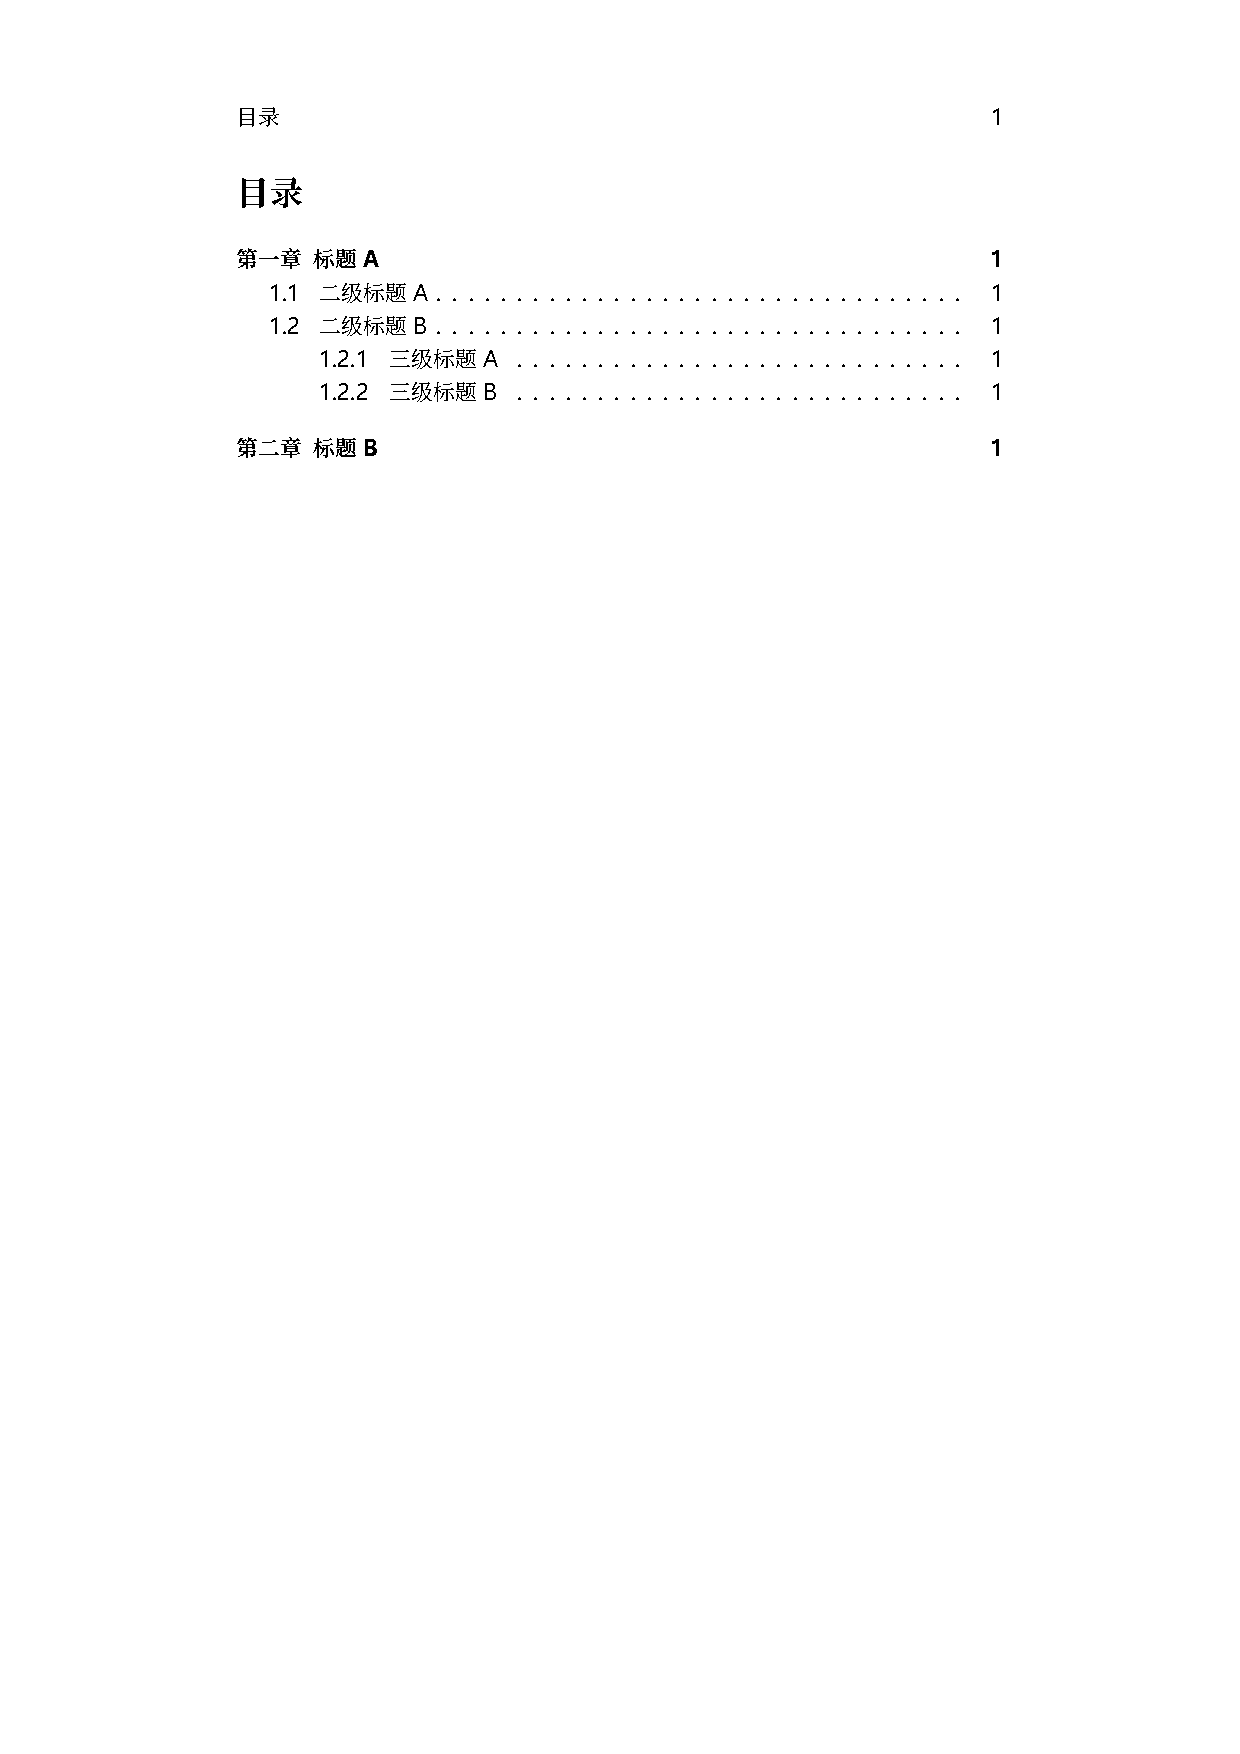
\includegraphics[page=1,clip,trim =0 {0.7\paperheight} 0 {0.1\paperheight},width=0.8\textwidth]{fig/section-tmp.pdf}
    %        \caption{Title}
    %        \label{fig:somthing}
        \end{figure}
    \end{texsepcode}
    \LaTeX{}需要编译两次\footnote{实际上所有的具有引用性质的内容都需要编译两次才可以正常的显示出来,另外有一些需要跨页的(如longtable),也需要多次的编译才可以正常的显示}才可以完整的将目录显示出来,因为\LaTeX{}必须通过第一遍编译获取所有目录的引用,才可以在下一次编译的时候添加新的目录。

    \subsection{定义目录深度}
    默认情况下目录只支持到\highunderline{subsubsection},如果需要增加目录深度,需要在序言位置就要使用以下的代码:
    
    \begin{texsepcode}
        \begin{texcodenoshad}
            \setcounter{tocdepth}{4}%设置目录级数
            \setcounter{secnumdepth}{4}%设置在几级目录前标记序号
        \end{texcodenoshad}
        \tcblower
        \begin{figure}[H]
            \centering
            \includegraphics[page=1,clip,trim =0 {0.7\paperheight} 0 {0.1\paperheight},width=0.8\textwidth]{\figpath{section-depth.pdf}}
        \end{figure}        
    \end{texsepcode}

    两行代码中的数字和\Ref{subsec:标题介绍}中备注的数字相同。

    数字的设置不必相同,互相并不矛盾,根据需要更改即可,其中\highunderline[hlyellow]{tocdepth}表明目录支持到几级深度,\highunderline[hlyellow]{secnumdepth}表明标题序号标记到几级深度。另外第一遍编译的时候可能会看到目录中增加了目录级数但是章节号并没有被添加,这是正常现象,完全更新会延迟到下一次编译。

    \subsection{添加标题引用}\label{sub:ref-in-title}
    使用\highunderline{hyperref}宏包后,生成的目录会自动添加到具体章节的链接和书签(如果没有该宏包则目录没有链接)。但是如果在文章内引用某章节,仍然需要为章节添加引用\footnote{该方法不局限于为章节添加引用,参考\Ref{sub:标签}}。

    为章节添加引用的方法是使用\highunderline{\textbackslash{}label{唯一标记}},该方法适用于任何你想引用某个位置的说明的地方,以本小节,其代码如下:
    \begin{texcode}
        \subsection{添加标题引用}\label{sub:ref-in-title}
    \end{texcode}

    在使用时,则需要使用\highunderline{\textbackslash{}ref}命令,如:
    \begin{texshow}
        在\ref{sub:ref-in-title}一节提到了如何对标题添加引用。
    \end{texshow}

    有时,不仅需要看到引用的序号,还想要知道相应的标题的名字。要完成这个需求,需要使用\highunderline{nameref}包:
    \begin{texshow}
        % \usepackage{nameref}
        如何对标题添加引用可以查看\ref{sub:ref-in-title}:\nameref{sub:ref-in-title}
    \end{texshow}

    如果嫌同时使用两个引用命令来完成上面的操作有些麻烦,可以通过重新定义一条引用命令\footnote{如何定义一条命令参考\Ref{sec:comm-envi}}的方法来合并引用(本手册即使用这种方法):
    \begin{texcode}
        \newcommand{\Ref}[1]{\ref{#1}:\nameref{#1}}
    \end{texcode}

    \begin{texshow}
        如何对标题添加引用可以查看\Ref{sub:ref-in-title}
    \end{texshow}
    
    
    \subsection{重新定义标题序号格式}
    有的时候会遇到需要自己定制标题序号的需求,对于中文环境和英文环境,相应的定制方式略有不同:

    \subsubsection{英文环境}
    英文环境,暂略(可以使用\highunderline{titlesec}系列宏包)
    % \todo{定义标题序号格式}
    \subsubsection{中文环境}
    中文环境要更改序号需要使用\highunderline{ctex}提供的命令,如下:
    \begin{texcode}
        \ctexset{
        section = {
            number = 第\chinese{section}章,
            format = \zihao{3}\bfseries,
        },
        subsection = {
            number = \arabic{section}.\arabic{subsection},
            format = \Large\bfseries
        },
        subsubsection = {
            number = \arabic{section}.\arabic{subsection}.\arabic{subsubsection},
            format = \Large\bfseries,
        },
    }
    \end{texcode}
    使用方法如上所示(这也是本手册使用的参数),每个级别的标题都可以分别自定义,其中\highunderline{number}表示序号的格式,相关的知识可以查看\Ref{subsub:number}的描述。\highunderline{format}表示每个标题的格式,相当于对每个标题添加什么样的命令。

    \subsection[更改目录标题]{更改目录中的标题文字}
    有的时候,因为标题过长,会导致目录不好看,这个时候,可以通过给标题添加参数的方式,定义显示在目录中的标题的内容。
    \begin{texcode}
        \section[短标题(显示在目录中的标题)]{长标题(显示在章节中的标题)}
        % 其他标题类方法同理
    \end{texcode}

    可以通过查看本节在目录和章节中的标题来认识其效果,其对应的代码为:
    \begin{texcode}
        \subsection[更改目录标题]{更改目录中的标题文字}
    \end{texcode}

    \subsection{取消标题序号}
    有的时候需要不显示标题的序号,只需要在命令后加$*$号即可。
    \begin{texcode}
        \section*{No Title Section}
    \end{texcode}

    但这时标题也不会出现的目录中,如果需要标题仍然在目录中出现需要在此处添加额外的声明,如下:
    \begin{texcode}
        \section*{No Title Section}\addcontentsline{toc}{section}{Title of the section} 
        %三个参数分别表示添加的位置是\highunderline{正文目录(toc)},级别是\highunderline{section},目录中显示的文字是\highunderline{Title of the section}
    \end{texcode}
    其中,\highunderline{\textbackslash{}addcontentsline}命令还可以用于添加其他类型的目录,如表格(第一个参数为\highunderline{lot}),图片(\highunderline{lof})等,但并不是很常用。

    \subsubsection*{取消标题序号的演示}\addcontentsline{toc}{subsubsection}{取消标题序号的演示} 
    使用代码如下,注意添加后会在目录中失去页码的引用:
    \begin{texcode}
        
        \subsubsection*{取消标题序号的演示}
        \addcontentsline{toc}{subsubsection}{取消标题序号的演示} 
    \end{texcode}